\documentclass[12pt]{article}
\usepackage[margin=2.5cm]{geometry}
\usepackage{enumerate}
\usepackage{amsfonts}
\usepackage{amsmath}
\usepackage{fancyhdr}
\usepackage{amsmath}
\usepackage{amssymb}
\usepackage{amsthm}
\usepackage{mdframed}
\usepackage{graphicx}
\usepackage{subcaption}
\usepackage{adjustbox}
\usepackage{listings}
\usepackage{xcolor}
\usepackage{booktabs}
\usepackage[utf]{kotex}
\usepackage{hyperref}

\definecolor{codegreen}{rgb}{0,0.6,0}
\definecolor{codegray}{rgb}{0.5,0.5,0.5}
\definecolor{codepurple}{rgb}{0.58,0,0.82}
\definecolor{backcolour}{rgb}{0.95,0.95,0.92}

\lstdefinestyle{mystyle}{
    backgroundcolor=\color{backcolour},
    commentstyle=\color{codegreen},
    keywordstyle=\color{magenta},
    numberstyle=\tiny\color{codegray},
    stringstyle=\color{codepurple},
    basicstyle=\ttfamily\footnotesize,
    breakatwhitespace=false,
    breaklines=true,
    captionpos=b,
    keepspaces=true,
    numbers=left,
    numbersep=5pt,
    showspaces=false,
    showstringspaces=false,
    showtabs=false,
    tabsize=1
}

\lstset{style=mystyle}

\pagestyle{fancy}
\renewcommand{\headrulewidth}{0.4pt}
\lhead{Hyungmo Gu}
\rhead{CSC369 Week 11 Notes}

\begin{document}
\title{CSC369 Week 11 Notes}
\author{Hyungmo Gu}
\maketitle

\begin{itemize}
    \item Security
    \begin{itemize}
        \item Computer Security
        \begin{itemize}
            \item Techniques for \textbf{computing} in the presence of adversaries
            \item Four requirements of security
            \begin{enumerate}[1.]
                \item \textbf{Confidentiality:}
                \begin{itemize}
                    \item Preventing unauthorized release of info
                \end{itemize}
                \item \textbf{Integrity:}
                \begin{itemize}
                    \item Preventing unauthorized modification of info
                \end{itemize}
                \item \textbf{Availability:}
                \begin{itemize}
                    \item Ensuring access to legitimate users
                \end{itemize}
                \item \textbf{Authenticity:}
                \begin{itemize}
                    \item Verifying the identity of a user
                \end{itemize}
            \end{enumerate}

            \item Protection is about providing \underline{all of the above} on
            a single machine
            \begin{itemize}
                \item Is usually considered the responsibility of the OS
            \end{itemize}
        \end{itemize}
        \item Cryptography
        \begin{itemize}
            \item Techniques for communicating in the presence of adversaires
        \end{itemize}
    \end{itemize}
    \item Types of Threats
    \begin{enumerate}[1.]
        \item \textbf{Interception or eavesdropping:}
        \begin{itemize}
            \item Attacker gains knowledge tey should not have access to
            \item is attack on \textit{confidentiality}
            \item Reading or copying files that attacker should not have access to
            \item Intercepting network packets
        \end{itemize}

        \item \textbf{Modification:}
        \begin{itemize}
            \item Attacker alters existing files, programs, packets, etc.
            \item is attack on \textit{integrity}
            \item e.g. Starcraft map hack
        \end{itemize}

        \begin{center}
            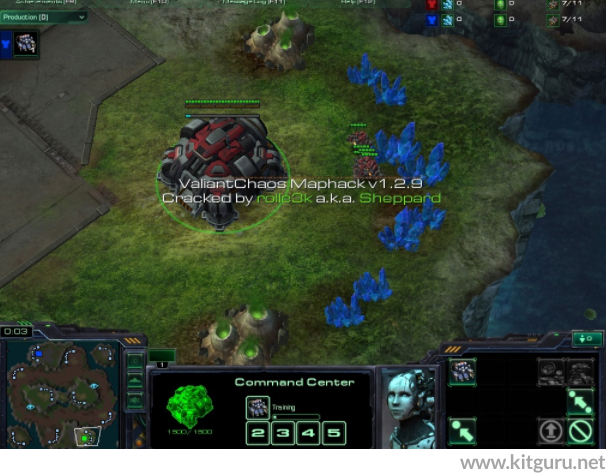
\includegraphics[width=0.8\linewidth]{images/week_11_notes_1_1.png}
        \end{center}
        \item \textbf{Theft of Service:}
        \begin{itemize}
            \item Happens when attacker installs daemon
            \item Is attack on \textit{availability}
            \item e.g. installing Daemon Tools Lite to run favourite Starcraft
            without CD Key (Don't do it!!)
        \end{itemize}

        \begin{center}
            
\includegraphics[width=0.3\linewidth]{images/week_11_notes_1_2.png}
        \end{center}
        \item \textbf{Fabrication:}
        \begin{itemize}
            \item Attacker creates counterfeit objects (files, messages, etc) which
            appears to come from a trusted source
            \item Is attack on \textit{authenticity}
            \item e.g. Fake Twitter website
        \end{itemize}

        \begin{center}
            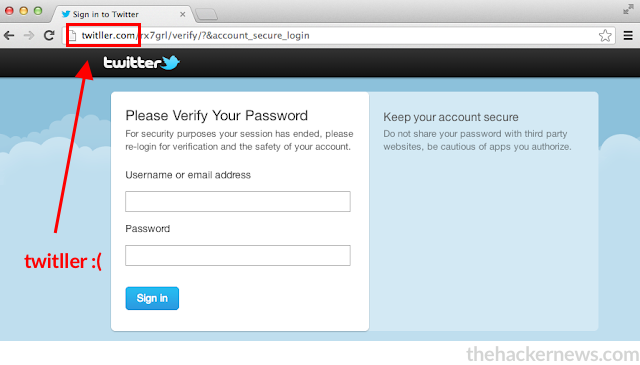
\includegraphics[width=0.8\linewidth]{images/week_11_notes_1_3.png}
        \end{center}
    \end{enumerate}
    \item Vulnerabilities in the System
    \begin{itemize}
        \item Physical Access
        \begin{itemize}
            \item Unauthorized physical acccess makes it a lot easier to gain
            unauthorized digital access
            \item e.g. Setting \textit{0000} as PIN number to Moe's Smartphone
        \end{itemize}
        \item Humans
        \begin{itemize}
            \item Who should you trust and how much?
            \item e.g. An employee giving others an access to Google's search
            algorithm source code
        \end{itemize}
        \item Operating Systems
        \begin{itemize}
            \item Flaws in the system allows security protocols to be circumvented
        \end{itemize}
        \item Networks
        \begin{itemize}
            \item Data treveling over unsecured communication lines, across multiple
            administrative domains
            \item e.g. Sending password data through HTTP, and not HTTPS (Data is sent without encryption)
        \end{itemize}
    \end{itemize}
    % \item Intrusion Detection
    \item Malicious Software (Malware)
    \begin{itemize}
        \item \textbf{Trap Doors}
        \begin{itemize}
            \item Is a program containing secret entry point that allows attacker
            to bypass security
        \end{itemize}
        \item \textbf{Logic Bombs}
        \begin{itemize}
            \item Is a peiece of code intentionally inserted into a software system
            that will set off a malicious function when specified conditions are met $^{[1]}$
            \item e.g. Viruses that activate on certain dates $^{[1]}$
        \end{itemize}
        \item \textbf{Trojan Horses}
        \begin{itemize}
            \item Misleads user of its true intent $^{[2]}$
            \item Tricks users into running it
            \item Gives full access to a stranger
            \item e.g. Fake Mac flash player $^{[3]}$
        \end{itemize}

        \begin{center}
            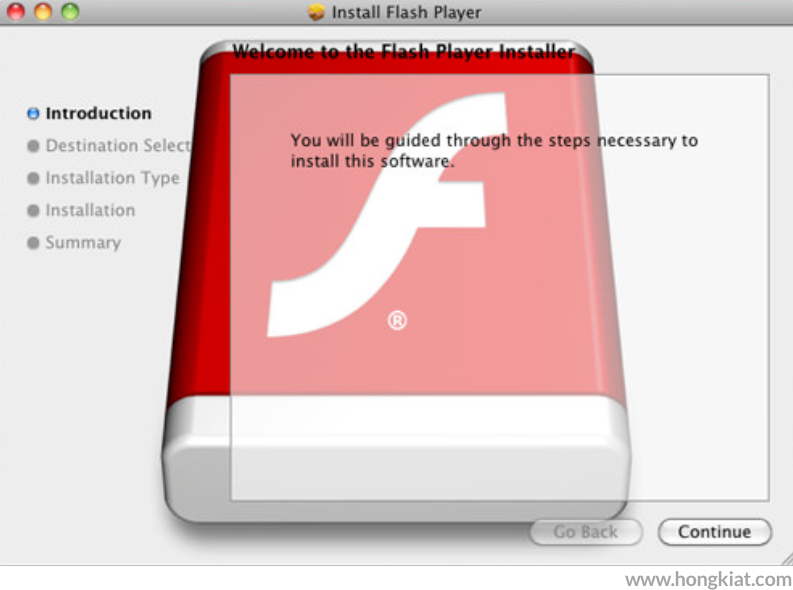
\includegraphics[width=0.8\linewidth]{images/week_11_notes_1_4.png}
        \end{center}
        \item \textbf{Viruses}
        \begin{center}
            \item Is a program that can ``infect'' other programs by copying itself
            onto them
        \end{center}
        \item \textbf{Worms}
        \begin{itemize}
            \item Is a program that spreads via network connections
            \item Relies on security failures on the target computer $^{[4]}$
            \item Uses infected machine as a host to scan and infect other computers $^{[4]}$
            \item Does not need to attach to another program like viruses
        \end{itemize}
    \end{itemize}

    \bigskip

    \underline{\textbf{References}}

    \bigskip

    \begin{enumerate}[1)]
        \item Wikipedia: Logic Bomb, \href{https://en.wikipedia.org/wiki/Logic_bomb}{link}
        \item Wikipedia: Trojan Horse, \href{https://en.wikipedia.org/wiki/Trojan_horse_(computing)}{link}
        \item Hongkiat: 10 Deadliest Computer Viruses of All Time, \href{https://www.hongkiat.com/blog/famous-malicious-computer-viruses/}{link}
        \item Wikipedia: Computer worm, \href{https://en.wikipedia.org/wiki/Computer_worm}{link}
    \end{enumerate}

    \item Stack \& Buffer Overflow Attacks
    \begin{itemize}
        \item Happens when a program writes more data to a buffer located on the
        stack than what is actually allocated $^{[1]}$
        \item Is most common means of gaining unauthorized access to a system

        \bigskip

        \underline{\textbf{Example:}}

        \bigskip

    \begin{lstlisting}[language=c]
    #include <string.h>

    void foo(char *bar)
    {
        char c[12]; // <- Overflow with value more than 12 characters in length

        strcpy(c, bar);  // no bounds checking
    }

    int main(int argc, char **argv)
    {
        foo(argv[1]);
        return 0;
    }
    \end{lstlisting}

    \bigskip

    \end{itemize}

    \begin{center}
        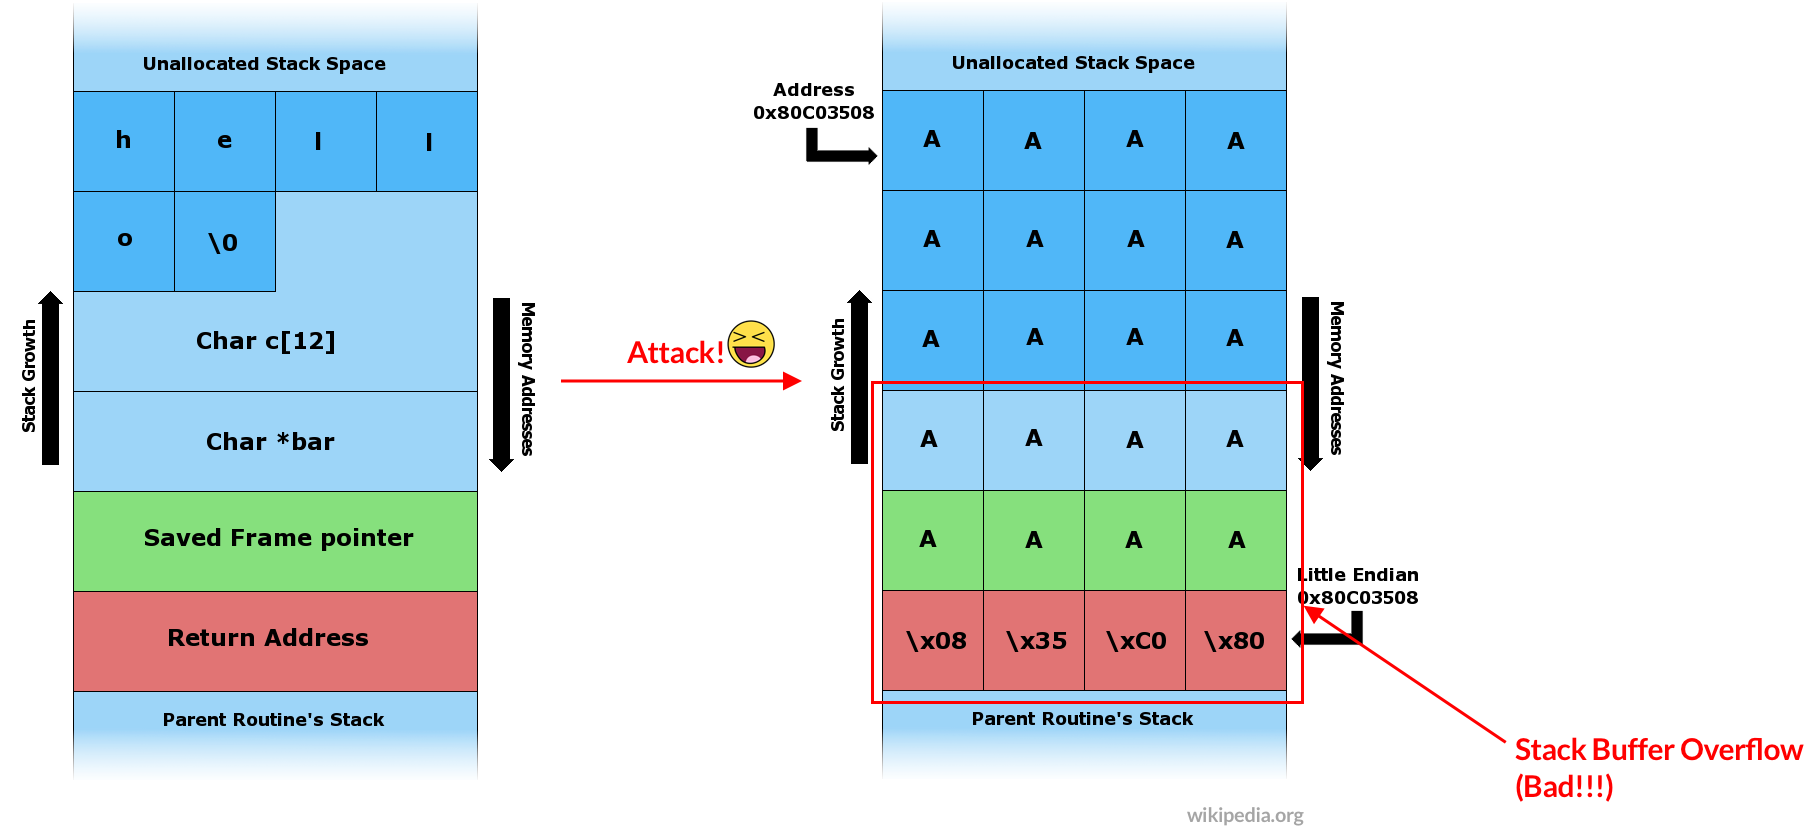
\includegraphics[width=\linewidth]{images/week_11_notes_1_5.png}
    \end{center}

    \bigskip

    \underline{\textbf{References}}

    \bigskip

    \begin{enumerate}[1)]
        \item Wikipedia: Stack buffer overflow, \href{https://en.wikipedia.org/wiki/Stack_buffer_overflow}{link}
    \end{enumerate}

    % \item Stack Attack
    % \item Trusted Computing Base (TCB)
    % \item Network Communications
    % \item Passive Network Attacks
    % \item Encryption Basics
    % \item More Passive Attacks
    % \item Active Network Attacks
    % \item Message Digests
    % \item Digital Signatures
    % \item One More Active Attack
    \item Security Design Principles
    \begin{itemize}
        \item Security is much, much more than just cryptography
        \item Still, system design is much an art as it is a science
        \begin{itemize}
            \item But decades of building systems the wrong way helped us
            gain some learned wisdom
        \end{itemize}
    \end{itemize}

    \item Princple of Least Privilege
    \begin{itemize}
        \item requires that in a particular layer of a computing environment, every
        (such as a process, a user, or a program) module must be able to access only
        the information and resources that are necessary for its legitimate purpose. $^{[1]}$
    \end{itemize}

    \bigskip

    \underline{\textbf{References}}

    \bigskip

    \begin{enumerate}[1)]
        \item Wikipedia: Principle of Least Privilege, \href{https://en.wikipedia.org/wiki/Principle_of_least_privilege}{link}
    \end{enumerate}
    % \item Protection Domains
    % \item Principle of Least-Common Mechanism
    % \item Protection Domains
    % \item Access Control Lists
    % \item Protection Domains
    % \item Outlook For The Future
    % \item Case Study: SSL
    \item SSL
    \begin{itemize}
        \item Means Secure Sockets Layer
        \item Is used to secure communications
        \item Is seen in web browsers (i.e. http:// $\to$ https://)
        \item Communication begins with a \textbf{handshake protocol}
        \begin{itemize}
            \item Requires \textbf{Certificate Authority} (CA)
            \item Web applications have a long list of CA's pre-installed
        \end{itemize}
    \end{itemize}

    \begin{center}
        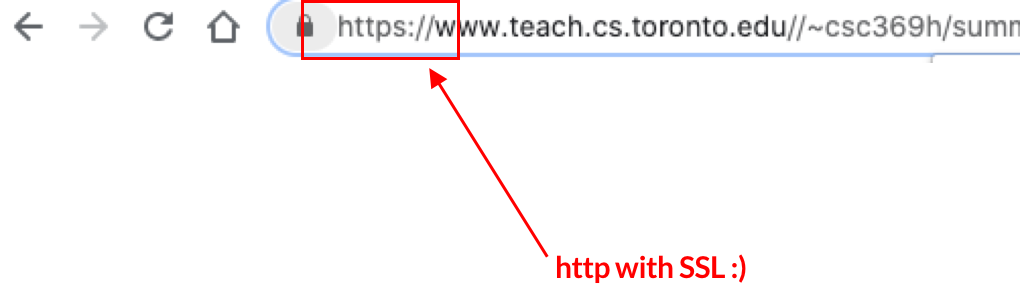
\includegraphics[width=\linewidth]{images/week_11_notes_1_6.png}
    \end{center}
    % \item SSL Handshake Protocol
    % \item If OSs were Beer
\end{itemize}

\end{document}